\documentclass{article}

\usepackage{polski}
\usepackage{amsmath}
\usepackage{graphicx}
\usepackage{float}
\usepackage{subfig}
\usepackage{multirow}

\title{Interpolacja według metody Hermite'a}
\author{\textbf{Łukasz Wala}\\
    \textit{AGH, Wydział Informatyki, Elektroniki i Telekomunikacji} \\
    \textit{Metody Obliczeniowe w Nauce i Technice 2021/2022}}
\date{Kraków, \today}

\begin{document}
\maketitle

\section{Opis problemu}
Główną ideą zadania jest zbadanie zachowania wielomianów interpolacyjnych
dla poniższej funkcji skonstruowanych metodą Hermite'a korzystając z różnego 
rozmieszczenia węzłów: równomiernie oddalonych oraz według pierwiastków wielomianu
Czebyszewa.

Badana funkcja:
\[f(x)=x^2-m\cdot\cos\left(\frac{\pi x}{k}\right)\]
\[f'(x) = 2x+\sin(\frac{\pi x}{k})\cdot\frac{m\pi}{k}\]
Gdzie $k=\frac{1}{2}$, $m=4$ oraz $x\in [-6,6]$.


\section{Opracowanie}
Do skonstruowania wielomianu użyty zostanie załączony program w języku Python. Zakres liczb węzłów, dla których
badane będą wielomiany wynosi 3-50, gdzie dla każdego węzła rozważana jest wartość funkcji w punkcie i jej pierwsza pochodna
(20 węzłów = 40 informacji).

\begin{figure}[H]
    \centering
    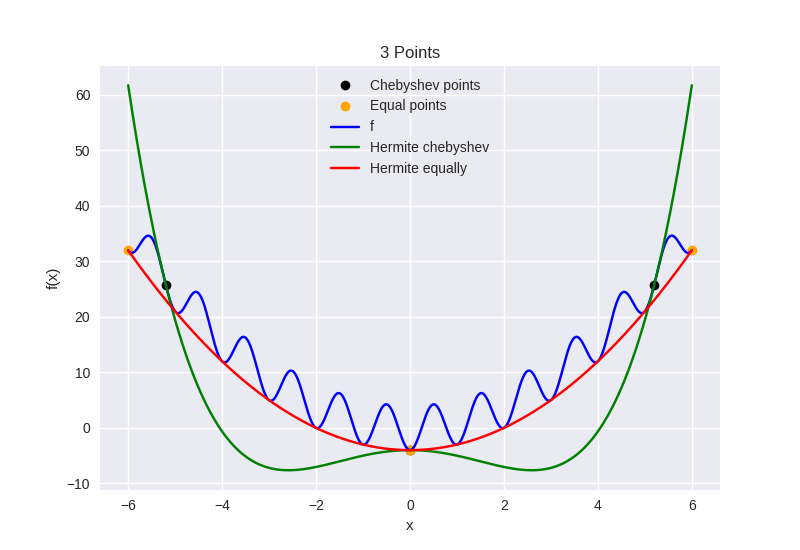
\includegraphics[width=0.8\textwidth]{img/herm_3.png}
    \caption{Metoda Hermite'a dla 3 punktów}
\end{figure}

\begin{figure}[H]
    \centering
    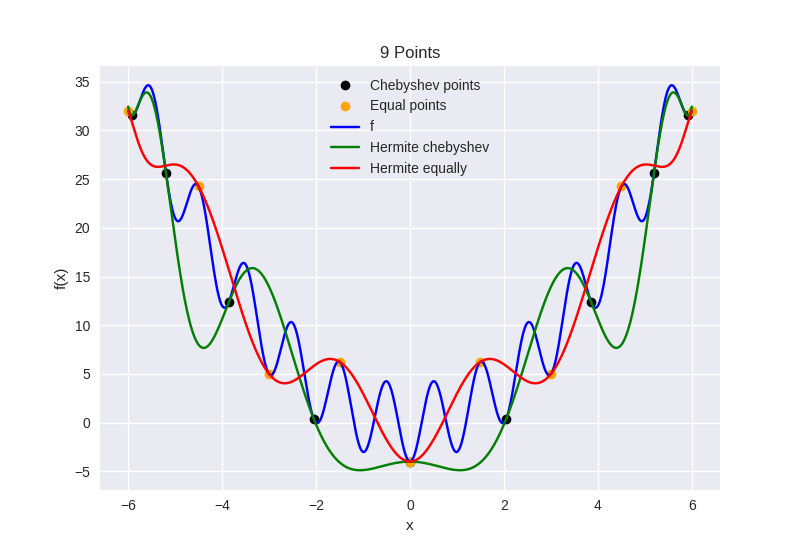
\includegraphics[width=0.8\textwidth]{img/herm_9.png}
    \caption{Metoda Hermite'a dla 9 punktów}
\end{figure}

Można zauważyć, że w węzłach zarówno wartości jak i pochodne (kierunek zmiany wawrtości funkcji jest wizualnie podobny,
są do siebie niejako styczne) są równe.

\begin{figure}[H]
    \centering
    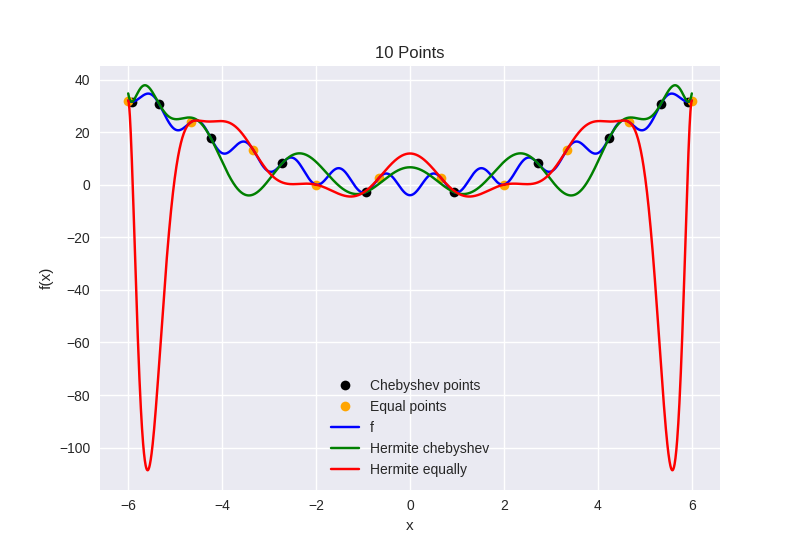
\includegraphics[width=\textwidth]{img/herm_10.png}
    \caption{Metoda Hermite'a dla 10 punktów - efekt Rungego}
\end{figure}

Dla 10 węzłów rozmieszczonych równomiernie zaczyna pojawiać się efekt Rungego, pogłębia się dla większych liczb węzłów.
Co za tym idzie, równomierne rozmieszczenie nie skutkuje zadowalającym przybliżeniem funkcji $f$. 
Dla punktów rozmieszczonych według węzłów Czebyszewa efekt nie występuje.

Poniżej wykresy już tylko dla rozmieszczenia według węzłów Czebyszewa:

\begin{figure}[H]
    \centering
    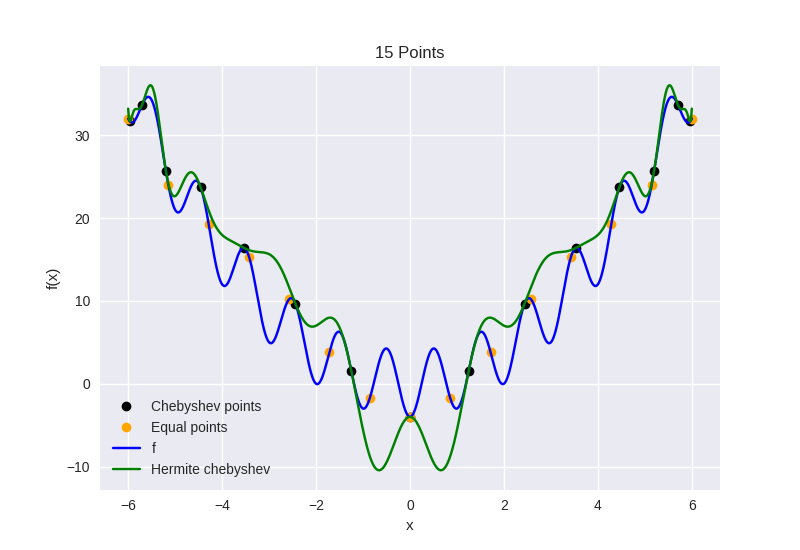
\includegraphics[width=\textwidth]{img/herm_15.png}
    \caption{Metoda Hermite'a dla 15 punktów}
\end{figure}

\begin{figure}[H]
    \centering
    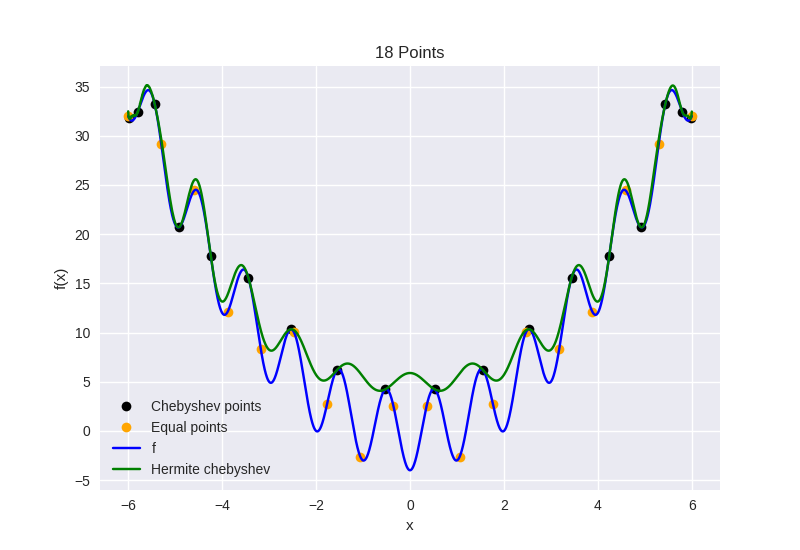
\includegraphics[width=\textwidth]{img/herm_18.png}
    \caption{Metoda Hermite'a dla 18 punktów}
\end{figure}

Na powyższych wykresach można zauważyć ciekawe zjawisko: dla nieparzystej ilości punktów środkowy zawsze występuje w punkcie 0, co
w połączeniu z faktem, że funkcja ma minimum lokalne w punkcie 0 (pochodna równa 0), sprawia, że dla wielomianu interpolacyjnego czasem
wystepuje tam również minimum (dobre przybliżenie), a czasem maksimum (słabe przybliżenie).

\begin{figure}[H]
    \centering
    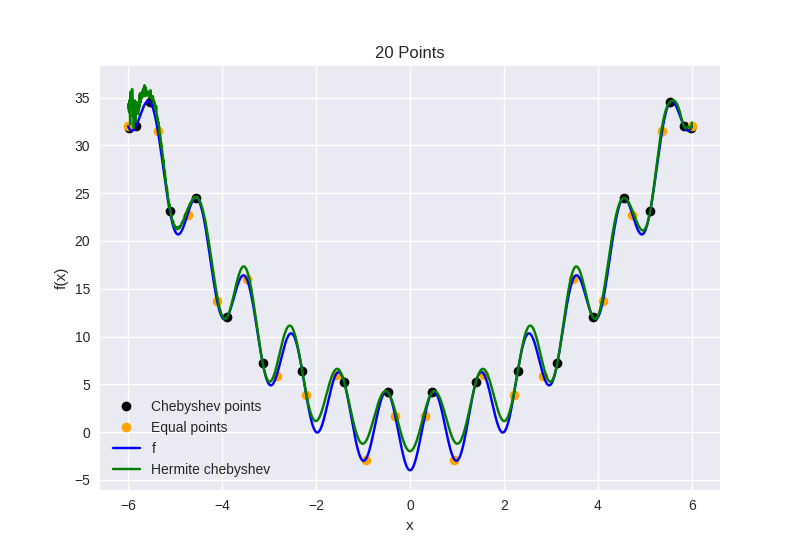
\includegraphics[width=\textwidth]{img/herm_20.png}
    \caption{Metoda Hermite'a dla 20 punktów}
\end{figure}

Dla 20 węzłów można zaobserwować (przy lewym krańcu przedziału) degradację jakości wielomianu i pojawiają się błędy (wielomian nawet
nie przechodzi przez punkty węzłów interpolacyjnych). Problemy te wynikają najprawdopodobniej z błędów obliczeń związanymi z precyzją
reprezentacji liczb zmiennoprzecinkowych.

\begin{figure}[H]
    \centering
    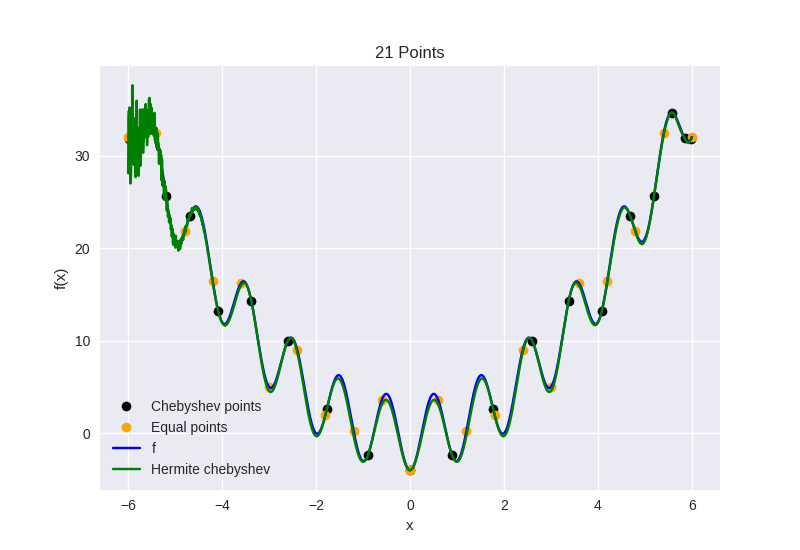
\includegraphics[width=0.8\textwidth]{img/herm_21.png}
    \caption{Metoda Hermite'a dla 21 punktów}
\end{figure}

Wraz ze zwiększaiem liczby węzłów efekt pogłębia się. Poniżej przykład dla 35 węzłów:

\begin{figure}[H]
    \centering
    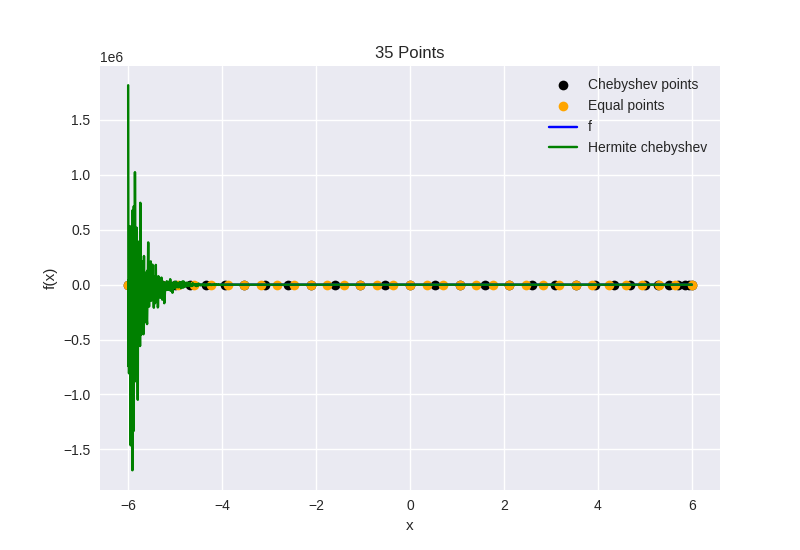
\includegraphics[width=0.8\textwidth]{img/herm_35.png}
    \caption{Metoda Hermite'a dla 35 punktów}
\end{figure}

\newpage
Pozostaje obliczenie dokładności i skonfrontowanie wyników z wnioskami uzyskanymi na podstawie wykresów. Miarami dokładności będą:
\begin{itemize}
    \item
    Średnia kwadratów odległości wartości wielomianu oraz funkcji $f$ dla 1000 równo oddalonych punktów,
    \item
    Maksymalna odległość wartości wielomianu oraz funkcji $f$ dla 1000 równo oddalonych punktów.
\end{itemize}


\begin{table}[H]
    \centering
    \begin{tabular}{|l|ll|ll|}
    \hline
    \multicolumn{1}{|c|}{\multirow{2}{*}{\begin{tabular}[c]{@{}c@{}}Liczba \\ węzłów\end{tabular}}} &
        \multicolumn{2}{c|}{Śred. kwadratów} &
        \multicolumn{2}{c|}{Maks. odległości} \\ \cline{2-5} 
    \multicolumn{1}{|c|}{} &
        \multicolumn{1}{c|}{Czebyszew} &
        \multicolumn{1}{c|}{rów. odd.} &
        \multicolumn{1}{c|}{Czebyszew} &
        \multicolumn{1}{c|}{rów. odd.} \\ \hline
    3 & \multicolumn{1}{l|}{158.169} &  23.976 & \multicolumn{1}{l|}{29.751} & 8.000 \\ \hline
    4 & \multicolumn{1}{l|}{419.003}  & 23.976  & \multicolumn{1}{l|}{39.794}  &  8.000 \\ \hline
    5 & \multicolumn{1}{l|}{24.093}  & 23.976  & \multicolumn{1}{l|}{9.990}  &  8.000 \\ \hline
    6 & \multicolumn{1}{l|}{81.197}  & 107.258  & \multicolumn{1}{l|}{18.078}  &  20.362 \\ \hline
    7& \multicolumn{1}{l|}{59.150}  & 23.976 & \multicolumn{1}{l|}{16.578}  &  8.000 \\ \hline
    8& \multicolumn{1}{l|}{94.262}  &  849.686 & \multicolumn{1}{l|}{25.812}  &  95.068 \\ \hline
    9& \multicolumn{1}{l|}{38.474}  & 17.230  & \multicolumn{1}{l|}{16.272}  &  7.985 \\ \hline
    10& \multicolumn{1}{l|}{46.306}  & 1532.943  & \multicolumn{1}{l|}{20.138}  &  143.211 \\ \hline
    11& \multicolumn{1}{l|}{46.427}  &  188494.398 & \multicolumn{1}{l|}{17.497}  &  1703.888 \\ \hline
    12& \multicolumn{1}{l|}{52.526}  &  2311475.213 & \multicolumn{1}{l|}{17.800}  &  6280.354 \\ \hline
    13& \multicolumn{1}{l|}{28.573}  &  23.976 & \multicolumn{1}{l|}{14.438}  &  8.000 \\ \hline
    14& \multicolumn{1}{l|}{33.156}  & 168221674  & \multicolumn{1}{l|}{14.867}  & 59270.349 \\ \hline
    15& \multicolumn{1}{l|}{27.904}  & 1877419731  & \multicolumn{1}{l|}{14.097}  & 207202.451  \\ \hline
    16& \multicolumn{1}{l|}{26.149}  &  6924927945 & \multicolumn{1}{l|}{19.712}  &  415272.937 \\ \hline
    17& \multicolumn{1}{l|}{21.467}  &  12966654597 & \multicolumn{1}{l|}{14.959}  & 590415.586  \\ \hline
    18& \multicolumn{1}{l|}{10.728}  & 14596394950 & \multicolumn{1}{l|}{9.883}  &  650177.679 \\ \hline
    19& \multicolumn{1}{l|}{3.225}  &  10846984985 & \multicolumn{1}{l|}{4.781}  &  580113.360 \\ \hline
    20& \multicolumn{1}{l|}{0.802}  &  5654153194 & \multicolumn{1}{l|}{4.002}  & 432505.466  \\ \hline
    21& \multicolumn{1}{l|}{0.408}  & 2158371055  & \multicolumn{1}{l|}{8.306}  &  275262.696 \\ \hline
    22& \multicolumn{1}{l|}{2.109}  & 623289078  & \multicolumn{1}{l|}{23.164}  &  152329.268 \\ \hline
    23& \multicolumn{1}{l|}{44.566}  & 139687143  & \multicolumn{1}{l|}{79.292}  &  74199.900 \\ \hline
    24& \multicolumn{1}{l|}{392.104}  &  24764958 & \multicolumn{1}{l|}{338.275}  &  32023.990 \\ \hline
    25& \multicolumn{1}{l|}{1566.757}  &  3564716 & \multicolumn{1}{l|}{561.743}  &  12462.642 \\ \hline
    26& \multicolumn{1}{l|}{51715.354}  &  402114 & \multicolumn{1}{l|}{2732.548}  &  4414.039 \\ \hline
    \end{tabular}
    \caption{Dokładności dla poszczególnych metod i rozmieszczeń}
\end{table}

Na podstawie tabeli dokładności można dojść do podobnych wniosków co w przypadku wykresów: dla równomiernego rozmieszczenia
węzłów dokładność rośnie do ok. 10 węzłów, potem zaczyna stale spadać, natomiast dla rozmieszczenia według węzłów Czebyszewa
dokładność rośnie do ok. 21 węzłów, dla większej liczby spada. Liczby węzłów, dla których osiągnięta została najlepsza dokładność
to: 21 (dla średniej kwadratów różnic) oraz 20 (dla maksimum odległości).


\section{Wnioski}
Metoda Hermite'a może posłużyć do przybliżania funkcji wielomianami interpolacyjnymi, kiedy, oprócz wartości punktów, znane
są pochodne w tych punktach. Do skutecznego przybliżenia muszą być zachowane pewne warunki: używanie węzłów Czebyszewa, żeby
uniknąć efektu Rungego, czy ograniczenie się do pewnej liczby węzłów, powyżej której występują błędy związane z operacjami
na liczbach zmiennoprzecinkowych.


\end{document}